\documentclass[12pt,a4paper]{article}
\usepackage{pdfpages}
\usepackage{booktabs}
\usepackage{helvet}
\usepackage{hyperref}
\usepackage{fancyhdr}


\hypersetup{
    colorlinks=true,
    linkcolor=purple,
    filecolor=magenta,      
    urlcolor=cyan,
    pdftitle={},
    pdfpagemode=FullScreen,
}

\begin{document}
\hyperref[contents]{}
\title{Higher Chemistry}
\author{Effective from}
\maketitle

\section{About this study aid}
This document has been designedto aid students studying the Higher Chemistry course in Scotland.
\section{}
\hyperlink{page.2}{View the table}

\newpage

\begin{table}[ht]
\begin{tabular}{@{}llllll@{}}
\toprule
TOPIC & 2022 & 2023 & 2024 & 2025 & 2026 \\ \midrule
Periodicity &  &  &  & \hyperlink{twentyfive.9}{22} &  \\
Structure and Bonding &  &  &  & \hyperlink{twentyfive.2}{1} &  \\
Oxidising and Reducing Agents &  &  &  & \hyperlink{twentyfive.2}{2,3}&  \\ \cmidrule(r){1-6}
Systematic Carbon Chemistry &  &  &  & 4, 8, 9 &  \\
Alcohols, Carboxylic acids, Esters, Fats and Oils &  &  &  & \hyperlink{twentyfive.3}{5},\hyperlink{twentyfive.3}{6} &  \\
Soaps, Detergents and Emulsifiers &  &  &  & 10, 11 &  \\
Proteins &  &  &  &  &  \\
Oxidation of Food &  &  &  &  &  \\
Fragrances &  &  &  & 12 &  \\
Skincare &  &  &  &  &  \\ \cmidrule{1-6}
Controlling the Rate &  &  &  & 13, 14, 19 &  \\
Getting the most from reactants &  &  &  & 20, 21 &  \\
Equilibria &  &  &  & 23 &  \\
Chemical Energy &  &  &  & 15, 17, 18 &  \\
Chemical analysis &  &  &  & 24, 25 &  \\ \cmidrule{1-6}
Open-ended &  &  &  &  &  \\
Problem solving &  &  &  &  &  \\ \bottomrule

\end{tabular}
\end{table}

\newpage
\pagestyle{fancy}
\fancyhf{}
\fancyhead[R]{\hyperlink{page.2}{\small Back to table}}
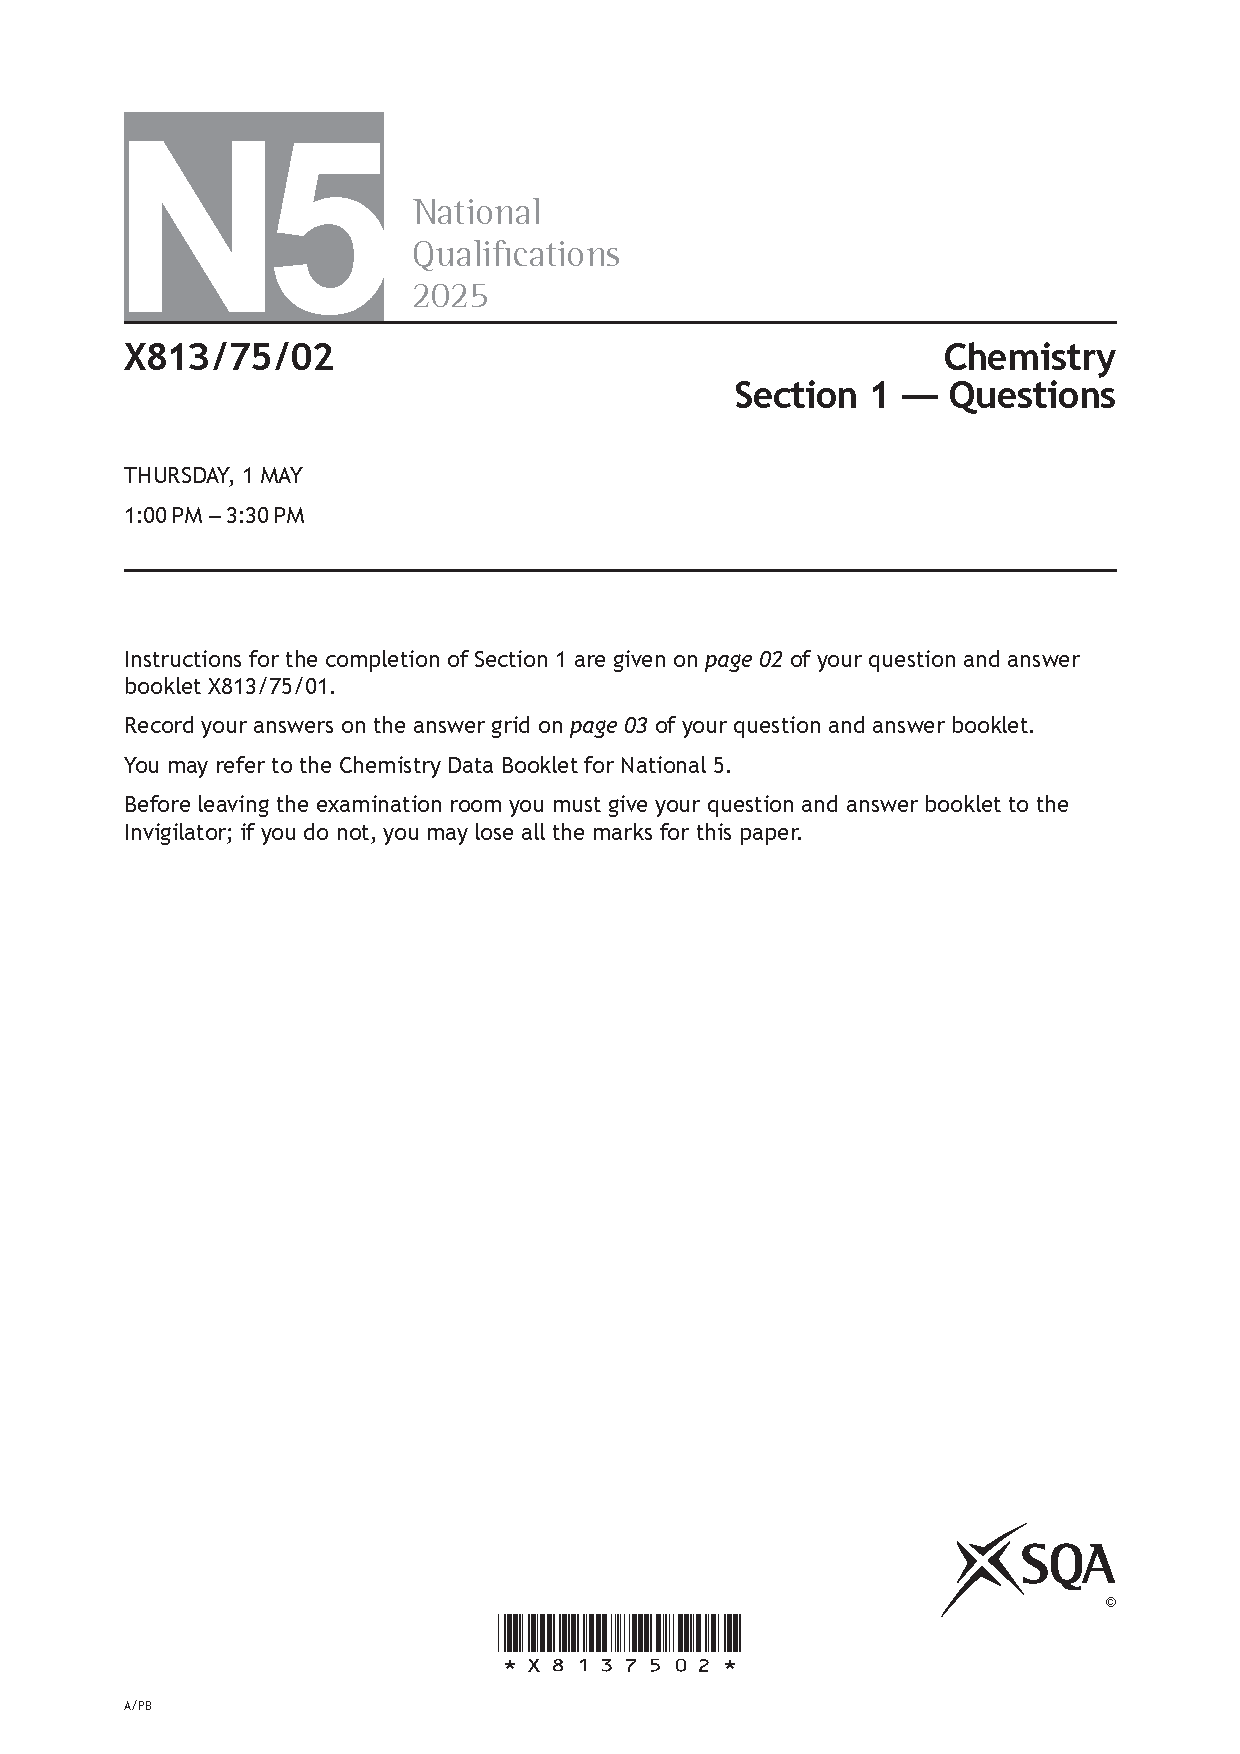
\includepdf[pages=1-56, link=true, linkname=twentyfive,
  pagecommand={\thispagestyle{fancy}}
]{2025.pdf}
\end{document}